\documentclass[tikz]{standalone}
%graphics
\usetikzlibrary{calc}

\begin{document}
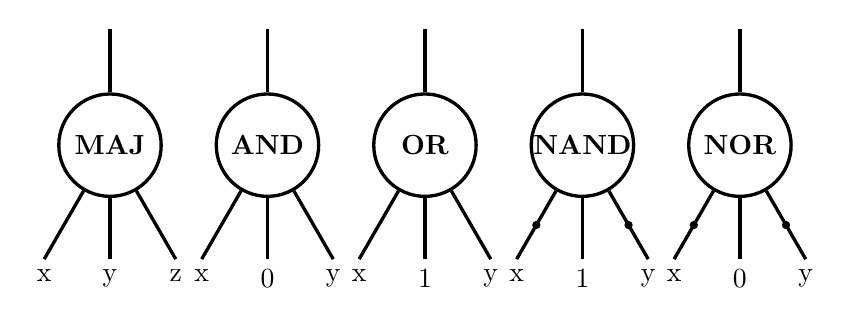
\begin{tikzpicture}[
very thick,
mnode/.style={
    circle,
    draw, 
    inner sep=0pt, 
    minimum size=1.3cm
    },
circ/.style={
    circle,
    fill,
    inner sep=0pt,
    minimum size=3pt,
    midway,
},
]
\begin{scope}
    \node[mnode] (maj) {\textbf{MAJ}};
    \draw(maj.north) -- ++(90:0.8cm);
    \draw(maj.240) -- ++(240:1cm)coordinate (x)node[below]{x};
    \draw(maj.-60) -- ++(-60:1cm)coordinate (z)node[below]{z};
    \draw(maj) -- ($(x)!.5!(z)$)coordinate(y)node[below]{y};
\end{scope}

\begin{scope}[xshift=2cm]
    \node[mnode] (maj) {\textbf{AND}};
    \draw(maj.north) -- ++(90:0.8cm);
    \draw(maj.240) -- ++(240:1cm)coordinate (x)node[below]{x};
    \draw(maj.-60) -- ++(-60:1cm)coordinate (y)node[below]{y};
    \draw(maj) -- ($(x)!.5!(y)$)node[below]{0};
\end{scope}

\begin{scope}[xshift=4cm]
    \node[mnode] (maj) {\textbf{OR}};
    \draw(maj.north) -- ++(90:0.8cm);
    \draw(maj.240) -- ++(240:1cm)coordinate (x)node[below]{x};
    \draw(maj.-60) -- ++(-60:1cm)coordinate (y)node[below]{y};
    \draw(maj) -- ($(x)!.5!(y)$)node[below]{1};
\end{scope}

\begin{scope}[xshift=6cm]
    \node[mnode] (maj) {\textbf{NAND}};
    \draw(maj.north) -- ++(90:0.8cm);
    \draw(maj.240) -- ++(240:1cm)node[circ]{} coordinate(x) node[below]{x};

    \draw(maj.-60) -- ++(-60:1cm)node[circ]{} coordinate(y) node[below]{y};
    \draw(maj) -- ($(x)!.5!(y)$)node[below]{1};
\end{scope}

\begin{scope}[xshift=8cm]
    \node[mnode] (maj) {\textbf{NOR}};
    \draw(maj.north) -- ++(90:0.8cm);
    \draw(maj.240) -- ++(240:1cm)node[circ]{} coordinate(x) node[below]{x};

    \draw(maj.-60) -- ++(-60:1cm)node[circ]{} coordinate(y) node[below]{y};
    \draw(maj) -- ($(x)!.5!(y)$)node[below]{0};
\end{scope}
\end{tikzpicture}
\end{document}